\chapter{Analiza problema}
Pronalazak visoko nelinearnih Booleovih funkcija je poznat problem na kojemu je provedeno mnogo istraživanja.
Težina problema dolazi od veličine prostora stanja, koji raste super eksponencijalno s porastom broja varijabli.
Općenito vrijedi da za $n$ varijabli Booleova funkcija ima $2^n$ elemenata u tablici istinitosti te postoji $2^{2^n}$ različitih Booleovih funkcija.
Eksponencijalni rast tablice istinitosti također predstavlja implementacijske probleme zbog memorijskih zahtjeva za zapis istoga, ali i vremenskih zahtjeva za računanje.
Osim velikog prostora stanja, problem je i količina visoko nelinearnih Booleovih funkcija, odnosno to što je njihov udio u svim Booleovim funkcijama određenog broja varijabli sve manji s porastom broja varijabli.
Tako primjerice za $4$ varijabli postoji ukupno $65536$ Booleovih funkcija, od čega su $896$ funkcije Bent-funkcije, što čini $1.3\%$ svih funkcija.
Sa $6$ varijabli postoji ukupno $1.84 \times 10^{19}$ različitih Booleovih funkcija, od čega su $5425430528$ funkcije Bent-funkcije, što čini svega $2.94 \times 10^{-8}\%$ svih funkcije.
Za $8$ varijabli ovaj omjer postaje još manji te je samo $8.155 \times 10^{-44}\%$ \cite{DiscoveryOfBent}.
Za broj Bent-funkcija vrijedi ograda dana u izrazu \eqref{eq:bent_num} \cite{CryptographicBooleanFunctions}.
\begin{equation}\label{eq:bent_num}
    \left(2^{\frac{n}{2}}\right)! 2^{2^{\frac{n}{2}}} \leq
    \#bent \leq
    2^{2^{n-1}-\frac{1}{2}\binom{n}{\frac{n}{2}}}.
\end{equation}
Ukupan broj Booleovih funkcija, kao i ograde i stvaran broj Bent-funkcija za određene brojeve varijabli dan je u tablici \ref{tbl:boolean_count}.
\begin{table}[]
\begin{tabular}{c|cccc}
$n$ & donja ograda & broj Bent-funkcija & gornja ograda & broj Booleovih funkcija \\ \hline
$2$ & $8$ & $8$ & $8$ & $8$ \\
$4$ & $384$ & $896$ & $2048$ & $65536$ \\
$6$ & $2^{23.3}$ & $2^{32.3}$ & $2^{38}$ & $2^{64}$ \\
$8$ & $2^{95.6}$ & $2^{106.3}$ & $2^{129.2}$ & $2^{256}$ \\
$10$ & $2^{262.2}$ & $?$ & $2^{612}$ & $2^{1024}$
\end{tabular}
\caption{Ukupan broj Booleovih funkcija i ograde za Bent-funkcije (podatci preuzeti iz \cite{CryptographicBooleanFunctions})}
\label{tbl:boolean_count}
\end{table}

\section{Mjere vrednovanja rješenja}
Uz sve spomenute probleme prilikom pronalaska nelinearnih Booleovih funkcija, dodatan problem javlja se prilikom vrednovanja rješenja.
Korišteni optimizacijski algoritmi temelje se na tome da svakom rješenju dodjeljuju vrijednost u skladu s time koliko je ono dobro ili loše te pomoću te informacije pronalaze nova, potencijalno bolja rješenja.
Ovisno o vrsti mjere vrednovanja, one mogu biti ili mjere odnosno funkcije dobrote ili funkcije kazne.
Funkcije dobrote rješenju pridjeljuju vrijednost na način da ono rješenje koje je bolje dobije veću vrijednost, dok funkcije kazne veću vrijednost dodjeljuju onom rješenju koje je lošije.
Ovisno o tome koja vrsta funkcija vrednovanja se koristi, optimizacijski problem se postavlja kao maksimizacijski u slučaju funkcija dobrote, odnosno minimizacijski u slučaju funkcija kazne.

Najjednostavnija korištena mjera vrednovanja rješenja je upravo iznos nelinearnosti funkcije $N_f$.
Navedena mjera pruža jednostavno tumačenje uspješnosti rješenja.
Problem ovako definirane funkcije dobrote je u tome što velik broj različitih Booleovih funkcija posjeduje jednaku razinu nelinearnosti, zbog čega je postoje velika područja u kojima optimizacijski algoritmi nemaju informaciju o tome napreduju li ka boljem rješenju.

Sljedeća korištena mjera vrednovanja je nadogradnja prethodne na način da se osim nelinearnosti 
Booleove funkcije također vrednuje i iznos drugog po veličini Walshovog koeficijenta.
Ideja ove mjere je iskoristiti svojstvo Walshovih koeficijenata da predstavljaju udaljenosti od pojedinih afinih Booleovih funkcija.
Na taj se način od više funkcija jednake nelinearnosti prednost daje onima čija je udaljenost od sljedeće najbliže afine funkcije maksimalna.
Time je povećana vjerojatnost da povećavanje udaljenosti od trenutno najbliže afine funkcije rezultira i povećanjem nelinearnosti, jer neovisno o tome je li udaljenost od sljedeće najbliže afine funkcije povećana ili smanjena, ona je minimalna s obzirom na do tada pronađena rješenja.
Dodatna motivacija za ovako definiranom mjerom vrednovanja je u tome što je poznato da Bent-funkcije imaju sve Walshove koeficijente jednakog iznosa, što znači da je prilikom traženja Bent funkcija cilj minimizirati sve Walshove koeficijente, gledano po njihovoj apsolutnoj vrijednosti.

Treća korištena mjera vrednovanja dana je izrazom \eqref{eq:cost_function}, koja je korištena u mnogim radovima, poput: \cite{MaximalNonlinearity}, \cite{CryptographicBoolean}, \cite{EvolvingBoolean} i \cite{picek2016new}.
\begin{equation}\label{eq:cost_function}
    cost = \sum_{\vec{w}\in \mathds{B}^n} \abs{\abs{W_f(\vec{w)}} - X}^R
\end{equation}
Navedena mjera je funkcija kazne, koja se temelji na sličnom principu prethodne mjere vrednovanja, samo što se umjesto najveća dva koeficijenta Walshovog spektra koriste svi koeficijenti.
Funkcija posjeduje poželjna svojstva u vidu kažnjavanja velikih vrijednosti Walshovih koeficijenata, uz mogućnost utjecaja na način kažnjavanja kroz parametre $X$ i $R$.
Premda spomenuti parametri predstavljaju mogućnost podešavanja funkcije kazne, oni također predstavljaju i problem s obzirom na to da uvode potrebu za pomnim odabirom istih te ispitivanje njihovog utjecaja na rad optimizacijskih algoritama.
Za potrebe ovog rada korištene su vrijednosti $R=3$ te $X=4$, koje su se pokazale kao najuspješnije u dosadašnjim radovima \cite{EvolvingBoolean}.

\section{Analiza susjedstva}
Prije nego li se primijene optimizacijski algoritmi, potrebno je proučiti problem, ne bi li se pronašle određene pravilnosti ili karakteristike rješenja, a na temelju čega se može unaprijediti rad optimizacijskih algoritama.
S tim ciljem napravljena je vizualizacija susjedstva na način da je napravljena dvodimenzionalna matrica, gdje element $a_{i, j}$ bojom odgovara hammingovoj udaljenosti Booleovih funkcija $f_i$ i $f_j$.
Opisani prikaz za slučaj funkcija s dvije varijable dan je na slici \ref{fig:function_2}. 
\begin{figure}[ht!] 
    \centering
    
\includegraphics[width=.4\textwidth]{img/function_2}
    \captionsetup{justification=centering}
    \caption{Prikaz susjedstva za funkcije dviju varijabli}
    \label{fig:function_2}
\end{figure}
Konačna boja polja u matrici dobivena je skaliranjem hammingovih udaljenosti na raspon od $0$ do $255$, te je tako dobiven broj korišten kao intenzitet sive boje.
Tako je primjerice na slici moguće primjetiti kako je glavna dijagonala crna, što je posljedica toga da ona prikazuje udaljenost funkcija od samih sebe, a ta udaljenost iznosi $0$, što rezultira crnom bojom.
Osim navedene glavne dijagonale, primjećuje se pravilnost i na sporednoj dijagonali, koja je naime u potpunosti bijela, što je posljedica toga da su to funkcije na najvećoj mogućoj udaljenosti.

\begin{figure}[!ht]
    \centering
    \begin{minipage}{.5\textwidth}
        \centering
        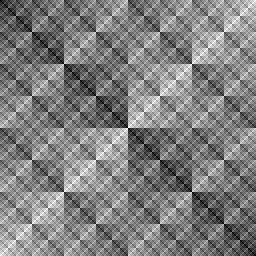
\includegraphics[width=.95\textwidth]{img/function_3}
        \captionsetup{justification=centering}
        \caption{Prikaz susjedstva za funkcije tri varijable}
        \label{fig:function_3}
    \end{minipage}%
    \begin{minipage}{.5\textwidth}
        \centering
        \includegraphics[width=.95\textwidth]{img/function_4}
        \captionsetup{justification=centering}
        \caption{Prikaz susjedstva za funkcije četiri varijable}
        \label{fig:function_4}
    \end{minipage}
\end{figure}

Na slici \ref{fig:function_3} grafički su prikazane udaljenosti funkcija tri varijable, dok slika \ref{fig:function_4} prikazuje udaljenosti za funkcije četiri varijable. 
Kako postoji ukupno $65536$ različitih Booleovih funkcija četiri varijable, nije moguće prikazati udaljenosti na prethodno opisano način jer bi tako dobivena slika zauzimala $4$GB prostora.
Kako bi dimenzije slike bile manje, umjesto da jedan slikovni element predstavlja udaljenost dviju funkcija, napravljeno je da jedan slikovni element predstavlja udaljenosti $8$ funkcija međusobno.
To je ostvareno na način da svaki element zapravo prikazuje aritmetičku sredinu onoga što bi prikazivalo područje od $8\times8$ elemenata u slici pune razlučivosti.

Na prikazanim slikama moguće je primjetiti određene pravilnosti.
Kao što je već spomenuto za sliku \ref{fig:function_2}, i na primjerima funkcija s većim brojem varijabli vrijedi to da je glavna dijagonala crna, dok je sporedna dijagonala bijela.
Osim toga, primjećuje se kako je sliku moguće podijeliti u kvadrate, tako je na primjer svaku sliku moguće podijeliti na $4$ kvadrata, svaki od tih kvadrata također je moguće podijeliti na $4$ daljnja kvadrata, i tako dalje.
Premda navedeno može djelovati kao potencijalno korisno svojstvo, isto je posljedica redoslijeda kojim su zapisane Booleove funkcije.
Na primjeru slike \ref{fig:function_3}, postoji ukupno $256$ različitih Booleovih funkcija.
Prvih $128$ funkcija ima $0$ kao prvi bit tablice istinitosti, dok drugih $128$ ima $1$ na mjestu prvog bita.
Ta promjena bita je razlog zbog kojeg je sliku moguće podijeliti na kvadrate upravo na mjestu gdje se mijenja vrijednost tog bita.
Manje kvadrate unutar slike moguće je objasniti na isti način, naime bit na drugom mjestu u tablici istinitosti imati će vrijednost $0$ za prve $64$ funkcije, nakon čega će imati vrijednost $1$ za sljedeće $64$ funkcija, nakon čega će opet imati vrijednost $0$ i tako dalje.
Ista pravilnost vrijedi za sve bitove tablice istinitosti, jedino što se frekvencija promjene vrijednosti bita povećava sa većim indeksima bita u tablici istinitosti.

\begin{figure}[ht!] 
    \centering
    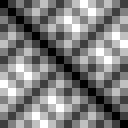
\includegraphics[width=.4\textwidth]{img/function_gray_2}
    \captionsetup{justification=centering}
    \caption{Prikaz susjedstva za funkcije dviju varijabli, za funkcije generirane korištenjem grayevog k\^oda}
    \label{fig:function_gray_2}
\end{figure}
Kako su sve uočene pravilnosti u prethodnim slikama posljedica načina na koji su generirane Booleove funkcije, isproban je grafički prikaz u kojemu funkcije nisu zapisane leksikografskim redom u odnosu na njihove tablice istinitosti, već korištenjem grayevog k\^oda.
Grayev k\^od je redoslijed zapisa Booleovih funkcija u kojemu se dvije susjedne funkcije uvijek razlikuju za točno jedan bit. 
Motivacija za prikazivanjem funkcija u ovom redoslijedu dolazi iz toga što su susjedne funkcije međusobno slične, zbog čega ne bi trebalo dolaziti do jednakih uzoraka udaljenosti kao u prethodnom zapisu.
Primjer na funkciji dvije varijable prikazan je na slici \ref{fig:function_gray_2}.

\begin{figure}[!ht]
    \centering
    \begin{minipage}{.5\textwidth}
        \centering
        
\includegraphics[width=.95\textwidth]{img/function_gray_3}
        \captionsetup{justification=centering}
        \caption{Prikaz susjedstva za funkcije tri varijable, za funkcije generirane korištenjem grayevog k\^oda}
        \label{fig:function_gray_3}
    \end{minipage}%
    \begin{minipage}{.5\textwidth}
        \centering
        \includegraphics[width=.95\textwidth]{img/function_gray_4}
        \captionsetup{justification=centering}
        \caption{Prikaz susjedstva za funkcije četiri varijable, za funkcije generirane korištenjem grayevog k\^oda}
        \label{fig:function_gray_4}
    \end{minipage}
\end{figure}


Slika \ref{fig:function_gray_3} prikazuje udaljenosti funkcija tri varijable, dok slika \ref{fig:function_gray_4} prikazuje udaljenosti funkcija četiri varijable.
Primjećuje se kako i u ovom redoslijedu zapisa funkcija postoje određene pravilnosti, točnije tamnija boja na dijagonalama.
Kao i kod leksikografskog poretka, glavna dijagonala je najtamnija jer prikazuje udaljenost funkcije od sebe same te je vrijednost tog polja $0$.
Sporedna dijagonala je također izrazito tamna, što je ponovno uzrokovano redoslijedom generiranja funkcija.
Naime, sporedna dijagonala prikazuje udaljenost dviju funkcija na međusobnoj udaljenosti $1$.
Sličan uzorak se ponavlja i na dijagonalama manjih kvadrata, dobivenih podjelom slike na četiri dijela.
Kako ni u ovom slučaju grafički prikaz nije omogućio pronalazak pravilnosti u svojstvima funkcija, osim redoslijeda kojim su generirane, ovi pristupi nisu korišteni u nastavku rada.

Osim grafičkih prikaza susjedstva, korisno je pogledati i funkcije grupirane na način da je za Booleovu funkciju prikazan popis svih Bent-funkcija koje su joj najbliže.
Motivacija tog prikaza je pronaći zajedničke dijelove najbližih Bent-funkcija te ustvrditi je li moguće odrediti koje bitove tablice istinitosti treba ili ne treba mijenjati kako bi se dobila funkcija veće nelinearnosti.
Prikaz Booleovih funkcija i njima najbližih Bent-funkcija za funkcije dvije varijable dan je u tablici \ref{tbl:neighbor}
\begin{table}[]
\centering
\begin{tabular}{ccccccccccc}
$0000$ & $0001$ &  & $0011$ & $0001$ &  & $0110$ & $1110$ &  & $0101$ & $0001$ \\
       & $0010$ &  &        & $0010$ &  &        & $0010$ &  &        & $1101$ \\
       & $0100$ &  &        & $1011$ &  &        & $0100$ &  &        & $0100$ \\
       & $1000$ &  &        & $0111$ &  &        & $0111$ &  &        & $0111$ \\
       &        &  &        &        &  &        &        &  &        &        \\
$1111$ & $1110$ &  & $1100$ & $1110$ &  & $1001$ & $0001$ &  & $1010$ & $1110$ \\
       & $1101$ &  &        & $1101$ &  &        & $1101$ &  &        & $0010$ \\
       & $1011$ &  &        & $0100$ &  &        & $1011$ &  &        & $1011$ \\
       & $0111$ &  &        & $1000$ &  &        & $1000$ &  &        & $1000$ \\
\end{tabular}
\caption{Popis Booleovih funkcija dvije varijable i njima najbližih Bent-funkcija}
\label{tbl:neighbor}
\end{table}
U danoj tablici primjećuje se pravilnost.
Točnije, svaka od prikazanih funkcija ima točno četiri Bent-funkcije koje su joj najbliže.
Usporede li se funkcije međusobno, primjećuje se da svaka funkcija ima par, odnosno drugu funkciju takvu da prva funkcija ima četiri njoj najbliže Bent-funkcije, dok druga funkcija ima druge četiri Bent-funkcije koje su joj najbliže.
Navedeni parovi funkcija su prikazani jedan ispod drugoga u tablici \ref{tbl:neighbor} te se primjećuje kako je jedna funkcija zapravo negacija druge funkcije.
Isto se primjećuje i za Bent-funkcije koje su najbliže navedenim funkcijama, gdje vrijedi da je Bent-funkcije najbliže prvoj funkciji moguće dobiti negiranjem Bent-funkcija najbližih drugoj funkciji.
Opisano svojstvo proizlazi iz definicije afinih Booleovih funkcija, dane u izrazu \eqref{eq:affine_definition}.
Ovisno o koeficijentu $a_0$, postoje dvije različite afine funkcije, jedna u kojoj je koeficijent $a_0$ jednak nuli, druga u kojoj je jednak jedinici.
Kako je koeficijent $a_0$ povezan operatorom XOR, on zapravo uzrokuje da za svaku afinu funkciju $f$, postoji afina funkcija $f'$ koja je jednaka negiranoj funkciji $f$.
Upravo iz tog razloga slijedi svojstvo da za svaku grupu funkcije i njoj pripadnih Bent-funkcija, postoji pripadna grupa dobivena negiranjem funkcija prethodne grupe.
Koristeći ovu činjenicu moguće je prostor pretrage smanjiti za pola, s obzirom da je dovoljno provjeriti jednu funkciju te ona ujedno daje informacije i za njoj komplementarnu funkciju.

Booleove funkcije dvije varijable korisne su za potrebe demonstracije jer ih je moguće sve prikazati, no ne pružaju vjeran uvid u problem, s obzirom na to da je točno pola funkcija afino, dok su preostale funkcije Bent-funkcije, s udaljenošću $1$ od najbliže afine funkcije.
Isti način grupiranja zato je primijenjen na Booleove funkcije četiri varijable.
Primjećuje se kako u ovom slučaju funkcije imaju različit broj Bent-funkcija koje su im najbliže, no postoje određene pravilnosti.

Najviše susjednih Bent-funkcija imaju upravo afine funkcije te vrijedi da svaka afina funkcija ima točno $448$ susjednih Bent-funkcija, što je pola od ukupnog broja Bent-funkcija četiri varijable.
Kod afinih funkcija vrijedi da promjena bilo kojeg bita tablice istinitosti povećava nelinearnost za jedan, zbog čega ove funkcije nisu korisne za daljnje razmaztranje.
Za funkcije čija je nelinearnost jednaka jedan, moguće je primijetiti kako imaju uvijek jednak broj Bent-funkcija koje su im najbliže, točnije $168$.
Zanimljivo je primijetiti kako je ovdije moguće uočiti pravilnosti, tako primjerice za funkciju \texttt{0101010101010100} vrijedi da promjena bilo kojeg bita vodi prema funkciji veće nelinearnosti, osim promjene zadnjeg bita, što dovodi do afine funkcije čija je nelinearnost jednaka nuli.
Primjećuje se kako sve ostale funkcije također dolaze u pravilnim grupama, tako postoje funkcije koje imaju ukupno $64$ najbliže Bent-funkcije, funkcije koje imaju $56$, $16$, $4$ i $1$ najbližu Bent-funkciju.
Za svaku grupu definiranu na opisan način vrijedi da postoji skupina bitova zajednička svim Bent-funkcijama, što znači da postoji skupina bitova unutar svake funkcije koju se ne smije mijenjati kako bi se postigla maksimalna moguća nelinearnost.
Zanimljivo je uočiti postojanje funkcija koje su svojevrsni lokalni optimum.
Na primjer, funkcija \texttt{0101000000001010} ima nelinearnost $4$, a promjenom bilo kojeg bita navedene funkcije dobiva se funkcija čija nelinearnost iznosi $3$.
Unatoč tome, navedena funkcija nije Bent-funkcija, odnosno postoje funkcije čija je nelinearnost veća.